\tableofcontents

\newpage


\section{Решение нелинейных уравнений}

\subsection{Метод хорд}

\subsubsection{Описание метода}
\underline{Суть метода:} функция \textit{y = f(x)} на отрезке \textit{[a,b]} заменяется хордой и в качестве приближенного
значения корня принимается точка пересечения хорды с осью абсцисс.


\underline{Алгоритм метода:}
\begin{enumerate}
    \item Найти $a$ и $b$ такие, что $a*b$<$0$
    \item Вычислить $x_0$:  $x_0$=$a_0$ - $\frac{b_0-a_0}{f(b_0)-f(a_0)}$$f(a_0)$
    \item Вычислить $f(x_0)$
    \item По критерию из п.1 выбрать новый интервал: $[a_0,x_0]$ или $[x_0,b_0]$
    \item Вычислить $x_1$ и т.д., пока $|x_i - x_{i-1}|>\epsilon$; $x_i$=$\frac{a_{i}f(b_i)-b_{i}f(a_i)}{f(b_i)-f(a_i)}$
    \item Получим приближённое значение корня $x^*$=$x_n$
\end{enumerate}

\subsubsection{Блок-схема численного метода}
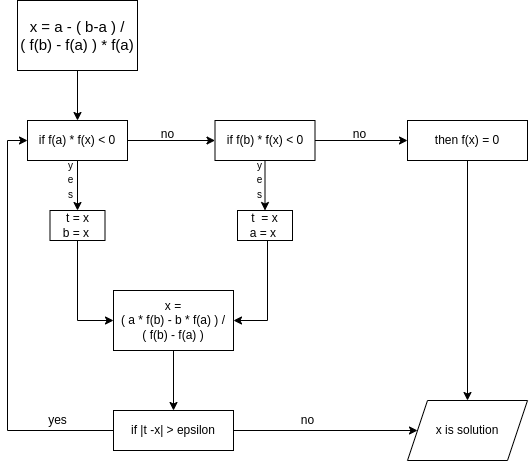
\includegraphics[scale=0.3]{img/block_2_chord}

\subsubsection{Listing реализованного численного метода}
\tiny
\begin{verbatim}
    public class CalculateEquationWithChordMethodRealization implements CalculateEquationWithChordMethod {
    
    @Override
    public double calculate(SimpleFunction func, double a, double b, double x, double epsilon, long n) {
        if (n == 0) {
            x = a - (b - a) / (func.apply(b) - func.apply(a)) * func.apply(a);
            n++;
            if (func.apply(a) * func.apply(x) < 0) {
                return calculate(func, a, x, x, epsilon, n);
            } else if (func.apply(b) * func.apply(x) < 0) {
                return calculate(func, x, b, x, epsilon, n);
            } else {
                return x;
            }
        } else {
            double x_i = (a * func.apply(b) - b * func.apply(a)) / (func.apply(b) - func.apply(a));
            n++;
            if (Math.abs(x_i - x) > epsilon) {
                x = x_i;
                if (func.apply(a) * func.apply(x) < 0) {
                    return calculate(func, a, x, x, epsilon, n);
                } else if (func.apply(b) * func.apply(x) < 0) {
                    return calculate(func, x, b, x, epsilon, n);
                } else {
                    return x;
                }
            } else {
                return x_i;
            }
        }
    }
}
\end{verbatim}
\normalsize
\newpage

\subsection{Метод простой итерации}

\subsubsection{Описание метода}
\underline{Суть метода:} Уравнение $f(x)$=0 приведём к эквивалентному виду: $x$=$\phi(x)$б выразив $x$ из исходного
уравнения.Если на отрезке локализации $[a,b]$ функция $\phi(x)$ определена, непрерывна и дифференцируема, то независимо
от выбора начального приближения $x_0$$\in$$[a,b]$ итерационная последовательность ${x_n}$ метода будет сходиться к корню
уравнения.


\underline{Алгоритм метода:} Сперва необходимо выразить функцию $x$=$\phi(x)$. Есть несколько способов это сделать, я выбрал
наиболее используемый и стабильный, где $\phi(x)$=$x$+$\lambda f(x)$, где $\lambda$=-$\frac{1}{\max_{[a,b]}|f(x)|}$\\
Далее, $x_i$ = $\phi(x_{i-1})$. Выполняем итерации до тех пор, пока $|x_i - x| > \epsilon$\\
В результате получим приближённое значение корня $x^*$=$x_n$.

\subsubsection{Блок-схема численного метода}
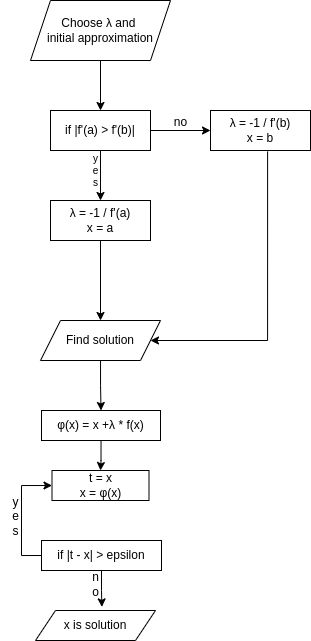
\includegraphics[scale=0.4]{img/block_2_iter}

\subsubsection{Listing реализованного численного метода}
\tiny
\begin{verbatim}
    public class CalculateEquationWithSimpleIterationsMethodRealization implements CalculateEquationWithSimpleIterationsMethod {

    @Override
    public double[] chooseLyambdaAndX_0(SimpleFunction derivativeFunc, double a, double b) {
        double v1 = Math.abs(derivativeFunc.apply(a));
        double v2 = Math.abs(derivativeFunc.apply(b));
        double v = (-1) * (1 / Math.max(v1, v2));
        if (v1 > v2) return new double[]{v, a};
        else return new double[]{v, b};
    }

    @Override
    public double calculate(SimpleFunction func, double lyambda, double x, double epsilon) {
        double x_i = x + lyambda * func.apply(x);
        if (Math.abs(x_i - x) <= epsilon) {
            return x_i;
        } else {
            return calculate(func, lyambda, x_i, epsilon);
        }
    }
}
\end{verbatim}
\normalsize

\newpage


\section{Решение систем нелинейных уравнений:}

\subsection{Метод Ньютона}

\subsubsection{Описание метода}
\underline{Алгоритм метода (на примере матрицы 2-го порядка):}
\begin{enumerate}
    \item Вычислить матрицу Якоби: $J(x,y)$=
    $\begin{vmatrix}
         \frac{\partial f_0(x_0 ... x_n)}{\partial x_0} & \ldots & \frac{\partial f(x_0 ... x_n)}{\partial x_n} \\
         \vdots                                         &        &                                              \\
         \frac{\partial f_n(x_0 ... x_n)}{\partial x_0} & \ldots & \frac{\partial g(x_0 ... x_n)}{\partial x_n} \\
    \end{vmatrix}$
    \item Решить СНАУ
    $\begin{vmatrix}
         \frac{\partial f_0(x_0 ... x_n)}{\partial x_0} & \ldots & \frac{\partial f(x_0 ... x_n)}{\partial x_n} \\
         \vdots                                         &        &                                              \\
         \frac{\partial f_n(x_0 ... x_n)}{\partial x_0} & \ldots & \frac{\partial g(x_0 ... x_n)}{\partial x_n} \\
    \end{vmatrix}$
    $\left(
    \begin{array}{c}
        \Delta x_0 \\
        \vdots     \\
        \Delta x_n \\
    \end{array}
    \right)$
    = --$\left(
    \begin{array}{c}
        f_0(x_0 ... x_n) \\
        \vdots           \\
        f_n(x_0 ... x_n) \\
    \end{array}
    \right)$
    , относительно \\ $\Delta x_0$ ... $\Delta x_n$
    \item А далее вычислять на каждой итерации: $x_{i+1}$=$x_i$+$\Delta x_i$ и $y_{i+1}$=$y_i$+$\Delta y_i$, где
    $x_i$, $y_i$ - текущее приближение к корню, $x_{i+1}$, $y_{i+1}$ - последующее приближение, $\Delta x$, $\Delta y$ -
    приращения к очередным приближениям.
    \item Процесс вычисления заканчивается при выполнении условий $|x_{i+1} - x_i|$ $\leq$ $\epsilon$, $|y_{i+1} - y_i$|$\leq$ $\epsilon$
\end{enumerate}

\subsubsection{Блок-схема численного метода}
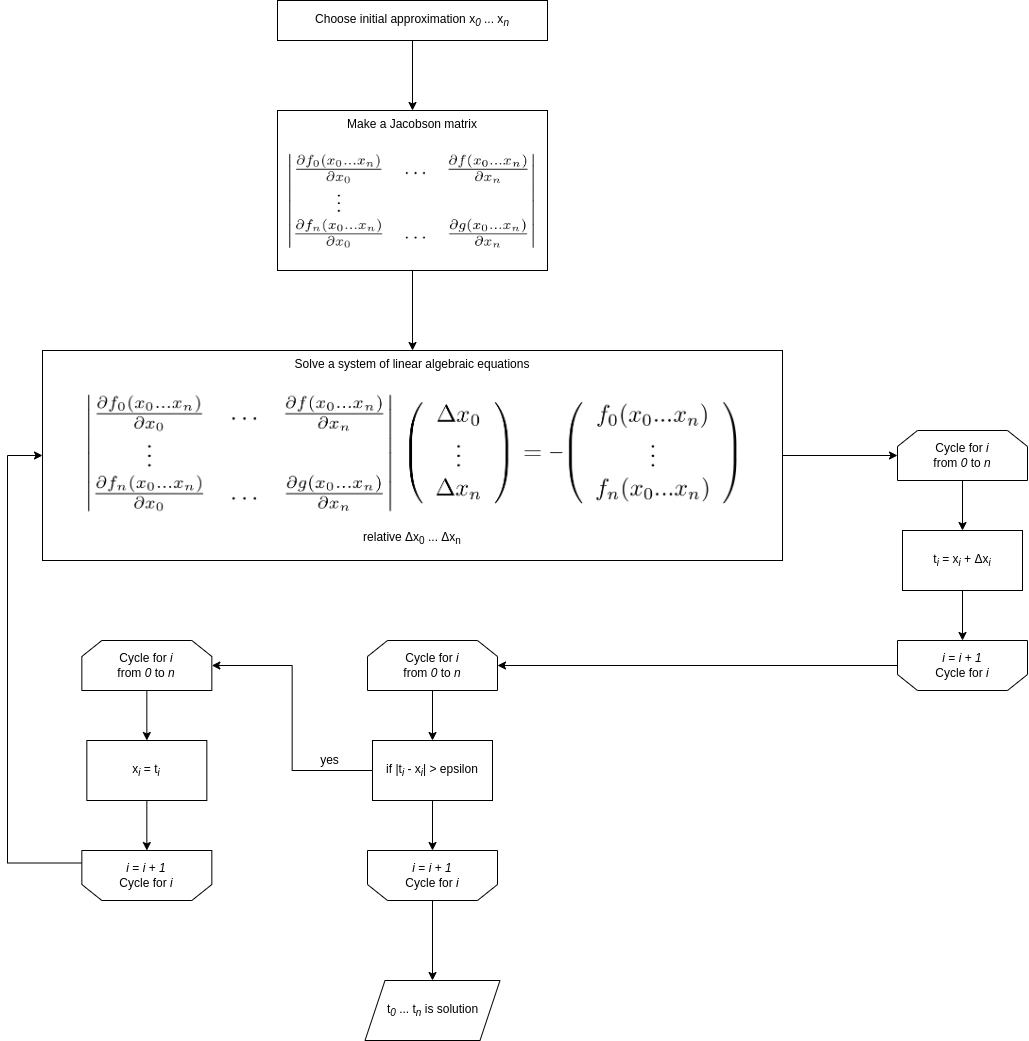
\includegraphics[scale=0.3]{img/block_2_newtone}

\subsubsection{Listing реализованного численного метода}
\tiny
\begin{verbatim}
    public class CalculateNSAEWithNewtonMethodRealization implements CalculateNSAEWithNewtonMethod {
    
    @Override
    public double[] calculate(double[] X, CreateMatrixForNewtoneMethod matrixCreator, double epsilon) throws MatrixCreateException, MatrixHasNoSolutionsException, TryCalculateNotDIagMatrixException {
        Matrix matrix = matrixCreator.create(X);
        MatrixCalulatorHandler calculator = new MatrixCalculatorHandlerImpl(matrix);
        calculator.transformToTriangleForm();
        double[] solutions = calculator.calcSolutions();
        double[] newX = new double[solutions.length];
        for (int i = 0; i < solutions.length; i++) {
            newX[i] = X[i] + solutions[i];
        }
        boolean flag = true;
        for (int i = 0; i < newX.length; i++) {
            if (Math.abs(newX[i] - X[i]) > epsilon) {
                flag = false;
                break;
            }
        }
        if (flag) {
            return newX;
        } else {
            return calculate(newX, matrixCreator, epsilon);
        }
    }
}
\end{verbatim}
\normalsize


\section{Examples}
\tiny
\begin{verbatim}
Enter "1" to solve the equation, enter "2" for NSAE:
\end{verbatim}\textbf{1}\begin{verbatim}
Choose the equation that you want to solve:
1. f(x) = sin(x)
2. f(x) = cos(x)
3. f(x) = x² - 1
4. f(x) = x³ - x + 4
5. f(n) = 2^n - 1
\end{verbatim}
\textbf{2}
\begin{verbatim}
The solution obtained by the chord method: 1.570783521943903
The solution obtained by the method of simple iterations: 4.712645995323825
\end{verbatim}

\begin{verbatim}
Enter "1" to solve the equation, enter "2" for NSAE:
\end{verbatim} \textbf{2} \begin{verbatim}
Choose the NSAE that you want to solve:
1.  x² + y² - 4 = 0
    -3x² + y = 0

2.  cos(x) - y = 0
    sin(y) - x = 0
\end{verbatim}
\textbf{1}
\begin{verbatim}
Solutions: x1 = 0.7832125666191059
           x2 = 1.8402657654730223
\end{verbatim}
\normalsize


\section{Вывод}
\subsection{Достоинства и недостатки метода хорд}
\subsubsection{Достоинства:}
\begin{itemize}
    \item Простота реализации
\end{itemize}
\subsubsection{Недостатки:}
\begin{itemize}
    \item Скорость сходимости - линейная.
    \item Зависит от выбора начального приближения.
\end{itemize}

\subsection{Достоинства и недостатки метода простой итерации:}
\subsubsection{Достоинства:}
\begin{itemize}
    \item Простота
\end{itemize}
\subsubsection{Недостатки:}
\begin{itemize}
    \item Сходимость в малой окрестности корня и вытекающая отсюда необходимость выбора начального приближения к корню
    из этой малой окрестности. В противном случае итерационный процесс расходится или сходится к другому корню этого уравнения.
    \item Если |$\phi '(x)$| $\approx$ 1, то сходимость может быть очень медленной.
\end{itemize}
\subsection{Достоинства и недостатки метода Ньютона:}
\subsubsection{Достоинства:}
\begin{itemize}
    \item Квадратичная сходимость.
\end{itemize}
\subsubsection{Недостатки:}
\begin{itemize}
    \item Важен удачный выбор начального приближения для обеспечения хорошей сходимости.
    \item Сходимость ухудшается с увеличением числа уравнений системы.
\end{itemize}